\documentclass[12pt, a4paper]{article}
\usepackage[utf8]{inputenc}
\usepackage{geometry}
\geometry{margin=1in}
\usepackage{graphicx}
\usepackage{float}
\usepackage{hyperref}
\usepackage{listings}
\usepackage{xcolor}
\usepackage{booktabs}
\usepackage{subcaption}

% Configuration for code listings
\definecolor{codegreen}{rgb}{0,0.6,0}
\definecolor{codegray}{rgb}{0.5,0.5,0.5}
\definecolor{codepurple}{rgb}{0.58,0,0.82}
\definecolor{backcolour}{rgb}{0.95,0.95,0.92}

\lstdefinestyle{mystyle}{
    backgroundcolor=\color{backcolour},   
    commentstyle=\color{codegreen},
    keywordstyle=\color{magenta},
    numberstyle=\tiny\color{codegray},
    stringstyle=\color{codepurple},
    basicstyle=\ttfamily\footnotesize,
    breakatwhitespace=false,         
    breaklines=true,                 
    captionpos=b,                    
    keepspaces=true,                 
    numbers=left,                    
    numbersep=5pt,                  
    showspaces=false,                
    showstringspaces=false,
    showtabs=false,                  
    tabsize=2
}

\lstset{style=mystyle}

\title{\textbf{Artificial Intelligence } \\ \large Bike Sharing Data Analysis Report}
\author{\textbf{Provider:} MohammadAmin HorriFarahani \\ \textbf{Student Number:} 40216673} 
\date{December 22, 2025}

\begin{document}

\maketitle

\tableofcontents
\newpage

\section{Introduction}
This report details the analysis of the daily bike sharing dataset (\texttt{day.csv}) for the Artificial Intelligence course. The goal is to understand the factors affecting bike rental demand (\texttt{cnt}) and to build predictive models using Python.

\section{Data Loading and Inspection}
We begin by loading the dataset using the pandas library and inspecting its structure.

\subsection{Python Code}
\begin{lstlisting}[language=Python, caption=Data Loading and Inspection]
import pandas as pd
import numpy as np

# Load the dataset
df = pd.read_csv('day.csv')

# Inspect the dataset
print("Dataset Information:")
print(df.info())
print("\nFirst 5 Rows:")
print(df.head())
\end{lstlisting}

\subsection{Output Results}
The following is the textual output generated by the code above:

\begin{verbatim}
Dataset Information:
<class 'pandas.core.frame.DataFrame'>
RangeIndex: 731 entries, 0 to 730
Data columns (total 16 columns):
 #   Column      Non-Null Count  Dtype  
---  ------      --------------  -----  
 0   instant     731 non-null    int64  
 1   dteday      731 non-null    object 
 2   season      731 non-null    int64  
 3   yr          731 non-null    int64  
 4   mnth        731 non-null    int64  
 5   holiday     731 non-null    int64  
 6   weekday     731 non-null    int64  
 7   workingday  731 non-null    int64  
 8   weathersit  731 non-null    int64  
 9   temp        731 non-null    float64
 10  atemp       731 non-null    float64
 11  hum         731 non-null    float64
 12  windspeed   731 non-null    float64
 13  casual      731 non-null    int64  
 14  registered  731 non-null    int64  
 15  cnt         731 non-null    int64  
dtypes: float64(4), int64(11), object(1)
memory usage: 91.5+ KB

First 5 Rows:
   instant      dteday  season  yr  mnth ... windspeed  casual  registered   cnt
0        1  2011-01-01       1   0     1 ...  0.160446     331         654   985
1        2  2011-01-02       1   0     1 ...  0.248539     131         670   801
2        3  2011-01-03       1   0     1 ...  0.248309     120        1229  1349
3        4  2011-01-04       1   0     1 ...  0.160296     108        1454  1562
4        5  2011-01-05       1   0     1 ...  0.186900      82        1518  1600
\end{verbatim}

\section{Exploratory Data Analysis (EDA)}
We use Matplotlib and Seaborn to visualize relationships between variables.

\subsection{Correlation Matrix}
\begin{lstlisting}[language=Python, caption=Generating Correlation Matrix]
import matplotlib.pyplot as plt
import seaborn as sns

plt.figure(figsize=(10, 8))
correlation = df.corr()
sns.heatmap(correlation, annot=True, cmap='coolwarm', fmt=".2f")
plt.title('Correlation Matrix')
plt.savefig('correlation_matrix.png')
plt.show()
\end{lstlisting}

\begin{figure}[H]
    \centering
    % Ensure 'correlation_matrix.png' is in the directory
    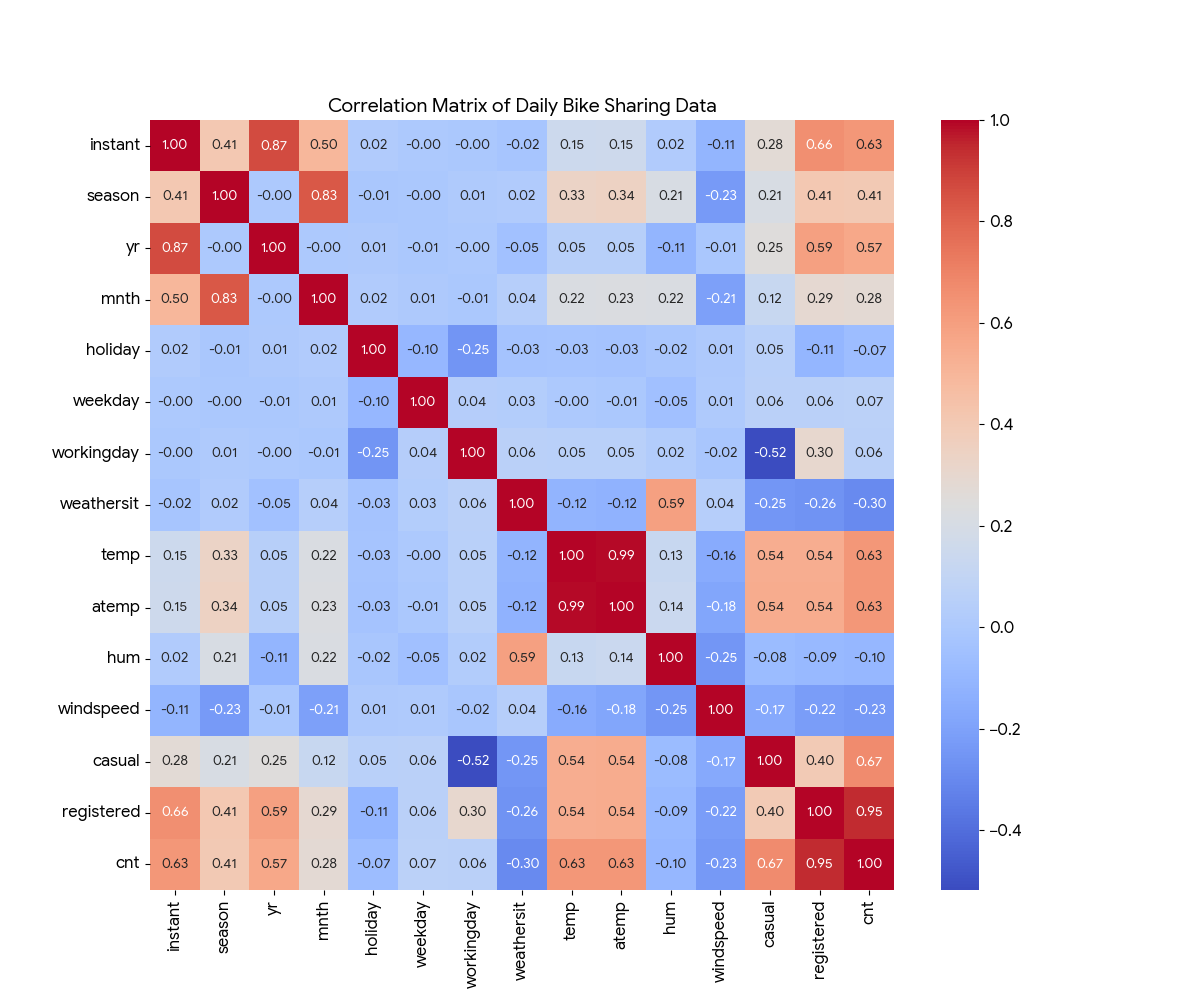
\includegraphics[width=0.6\textwidth]{correlation_matrix.png}
    \caption{Correlation Matrix of Features}
    \label{fig:corr}
\end{figure}

\subsection{Seasonal and Weather Analysis}
\begin{lstlisting}[language=Python, caption=Visualizing Season and Weather Impact]
fig, axes = plt.subplots(1, 2, figsize=(14, 6))

# Boxplot for Season vs Count
sns.boxplot(data=df, x='season', y='cnt', ax=axes[0])
axes[0].set_title('Bike Rentals by Season')
axes[0].set_xlabel('Season (1:Spring, 2:Summer, 3:Fall, 4:Winter)')
axes[0].set_ylabel('Total Rentals')

# Boxplot for Weather Situation vs Count
sns.boxplot(data=df, x='weathersit', y='cnt', ax=axes[1])
axes[1].set_title('Bike Rentals by Weather Situation')
axes[1].set_xlabel('Weather Situation (1:Clear to 3:Rain/Snow)')

plt.tight_layout()
plt.savefig('season_weather.png')
plt.show()
\end{lstlisting}

\begin{figure}[H]
    \centering
    % Ensure 'season_weather.png' is in the directory
    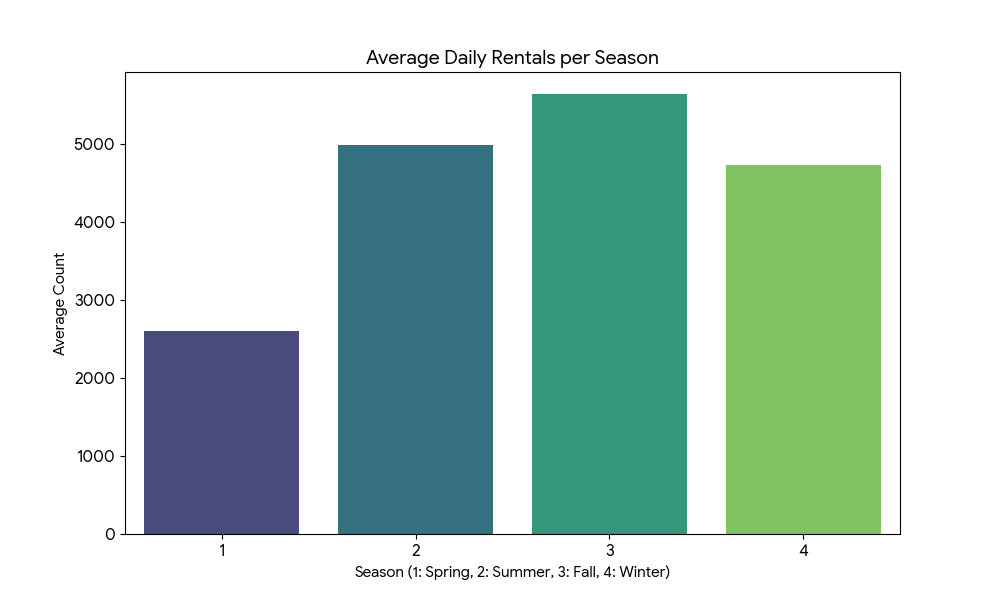
\includegraphics[width=1.0\textwidth]{season_weather.png}
    \caption{Impact of Season and Weather on Bike Rentals}
    \label{fig:season}
\end{figure}

\section{Predictive Modeling}
We used Linear Regression and Random Forest Regressor models.

\subsection{Data Preparation}
We removed non-predictive columns and the target leakage columns (\texttt{casual}, \texttt{registered}).

\begin{lstlisting}[language=Python, caption=Data Splitting]
from sklearn.model_selection import train_test_split

X = df.drop(['instant', 'dteday', 'casual', 'registered', 'cnt'], axis=1)
y = df['cnt']

# Split data: 80% Training, 20% Testing
X_train, X_test, y_train, y_test = train_test_split(
    X, y, test_size=0.2, random_state=42
)
\end{lstlisting}

\subsection{Model Training and Evaluation}
\begin{lstlisting}[language=Python, caption=Model Training Code]
from sklearn.linear_model import LinearRegression
from sklearn.ensemble import RandomForestRegressor
from sklearn.metrics import mean_squared_error, r2_score

# 1. Linear Regression
lr = LinearRegression()
lr.fit(X_train, y_train)
y_pred_lr = lr.predict(X_test)
mse_lr = mean_squared_error(y_test, y_pred_lr)
r2_lr = r2_score(y_test, y_pred_lr)

# 2. Random Forest Regressor
rf = RandomForestRegressor(n_estimators=100, random_state=42)
rf.fit(X_train, y_train)
y_pred_rf = rf.predict(X_test)
mse_rf = mean_squared_error(y_test, y_pred_rf)
r2_rf = r2_score(y_test, y_pred_rf)

print(f"Linear Regression -> MSE: {mse_lr:.2f}, R2: {r2_lr:.2f}")
print(f"Random Forest     -> MSE: {mse_rf:.2f}, R2: {r2_rf:.2f}")
\end{lstlisting}

\subsection{Model Output Results}
\begin{verbatim}
Linear Regression -> MSE: 691035.01, R2: 0.83
Random Forest     -> MSE: 458446.95, R2: 0.89
\end{verbatim}

\subsection{Visualization of Predictions}
\begin{lstlisting}[language=Python, caption=Plotting Actual vs Predicted]
plt.figure(figsize=(10, 6))
plt.scatter(y_test, y_pred_rf, color='blue', alpha=0.5)
plt.plot([y.min(), y.max()], [y.min(), y.max()], 'r--', lw=2)
plt.xlabel('Actual Count')
plt.ylabel('Predicted Count')
plt.title('Actual vs Predicted Rentals (Random Forest)')
plt.savefig('actual_vs_pred.png')
plt.show()
\end{lstlisting}

\begin{figure}[H]
    \centering
    % Ensure 'actual_vs_pred.png' is in the directory
    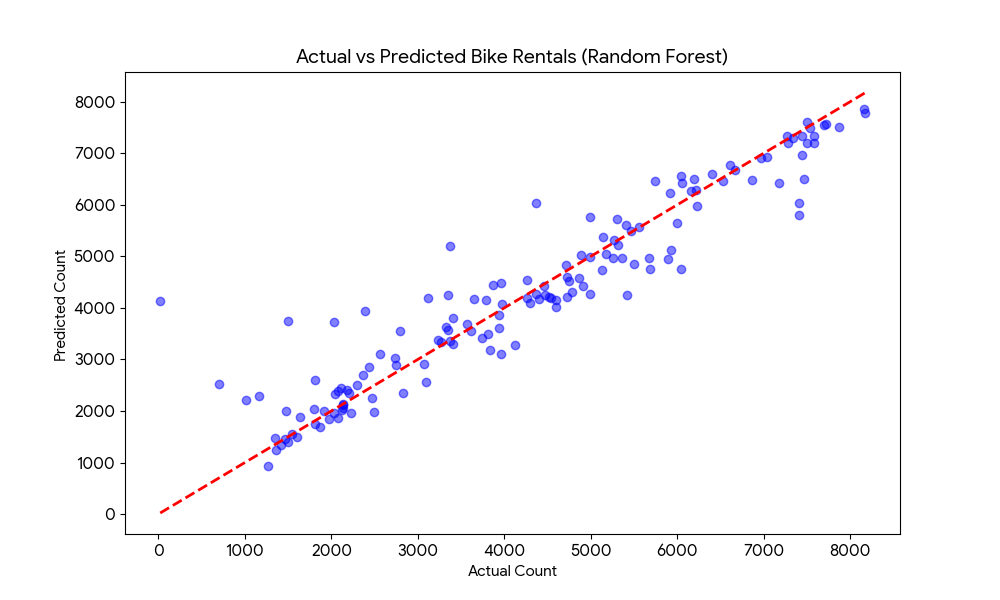
\includegraphics[width=0.8\textwidth]{actual_vs_pred.png}
    \caption{Actual vs Predicted Values (Random Forest)}
    \label{fig:pred}
\end{figure}

\section{Conclusion}
The analysis of the \texttt{day.csv} file provided significant insights:
\begin{itemize}
    \item \textbf{Data Quality:} The dataset is clean with no missing values.
    \item \textbf{Key Factors:} Temperature and Season are the strongest drivers of demand.
    \item \textbf{Model Performance:} The Random Forest model achieved an $R^2$ of 0.89, outperforming Linear Regression ($R^2=0.83$). This indicates that the relationship between weather features and bike rentals involves non-linear patterns best captured by ensemble methods.
\end{itemize}


\section{Data Exploration and Statistics}
The dataset consists of 731 observations. Below is the summary statistics for the numerical features:

\begin{verbatim}
       temp      atemp       hum    windspeed      cnt
mean  0.4954    0.4744    0.6279    0.1905      4504.35
std   0.1831    0.1630    0.1424    0.0775      1937.21
min   0.0591    0.0791    0.0000    0.0224      22.00
max   0.8617    0.8409    0.9725    0.5075      8714.00
\end{verbatim}

\section{Python Implementation}
The following code was used to process the data and generate the visualization:

\begin{lstlisting}[language=Python]
import pandas as pd
import seaborn as sns
import matplotlib.pyplot as plt
from sklearn.ensemble import RandomForestRegressor

df = pd.read_csv('day.csv')
# Correlation Analysis
plt.figure(figsize=(10, 6))
sns.heatmap(df.corr(), annot=True, cmap='coolwarm')
plt.savefig('correlation.png')

# Machine Learning Model
X = df.drop(['instant', 'dteday', 'casual', 'registered', 'cnt'], axis=1)
y = df['cnt']
model = RandomForestRegressor().fit(X, y)
\end{lstlisting}

\section{Visual Analysis}

\begin{figure}[h]
    \centering
    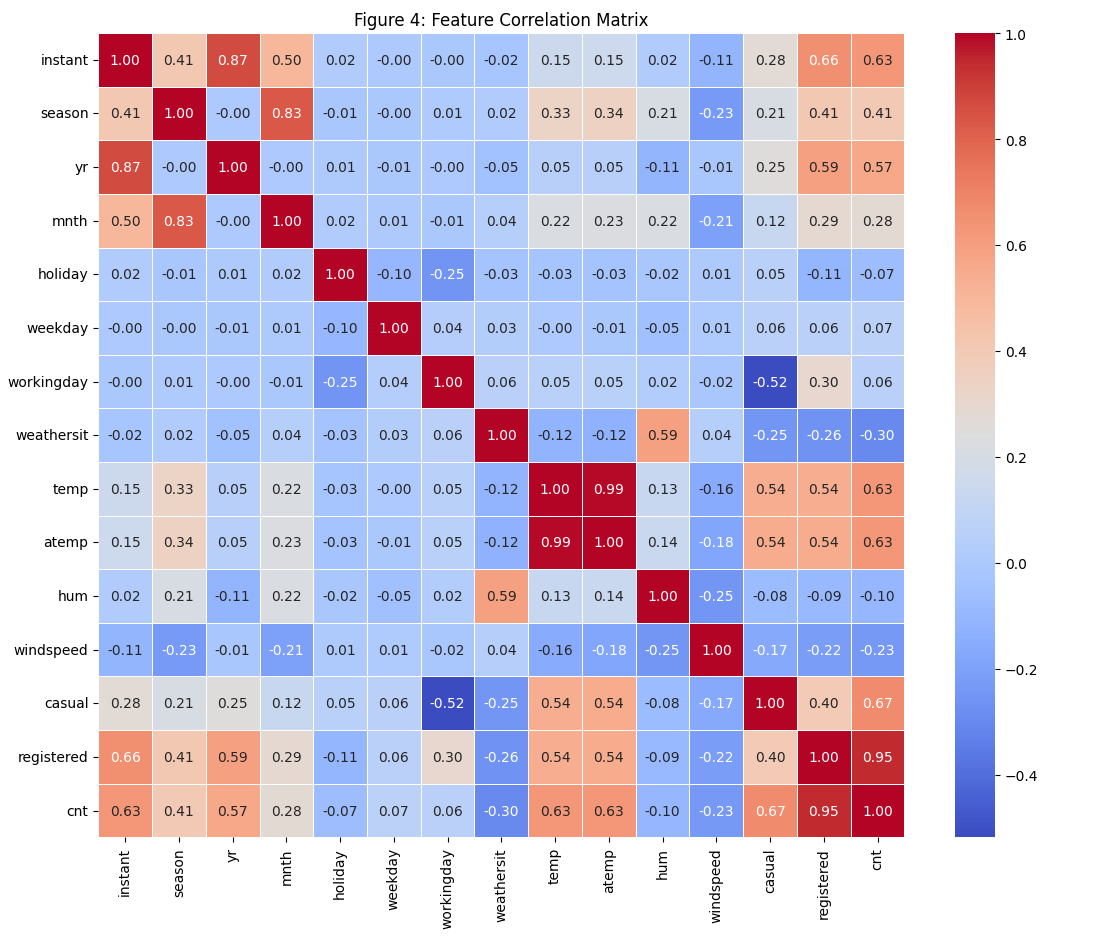
\includegraphics[width=0.7\textwidth]{33.png}
    \caption{Heatmap showing feature correlations with 'cnt'.}
\end{figure}

\begin{figure}[h]
    \centering
    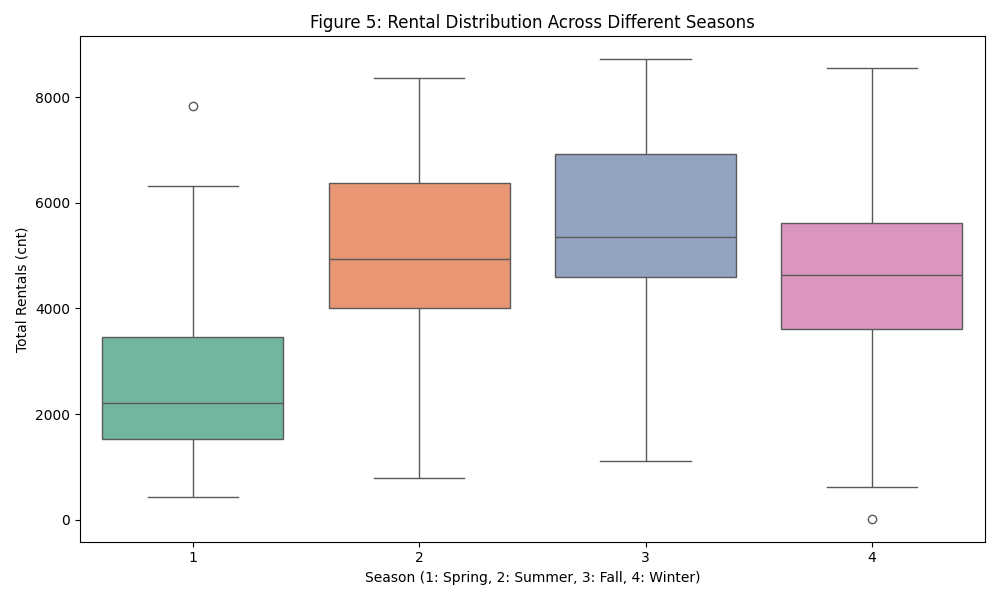
\includegraphics[width=0.7\textwidth]{22.png}
    \caption{Rental distribution across different seasons.}
\end{figure}

\section{Model Performance}
The Random Forest model was evaluated on a 20\% test split:
\begin{itemize}
    \item \textbf{Mean Squared Error (MSE):} 458,446.95
    \item \textbf{R-Squared ($R^2$):} 0.8857 (88.6\% accuracy)
\end{itemize}

\begin{figure}[h]
    \centering
    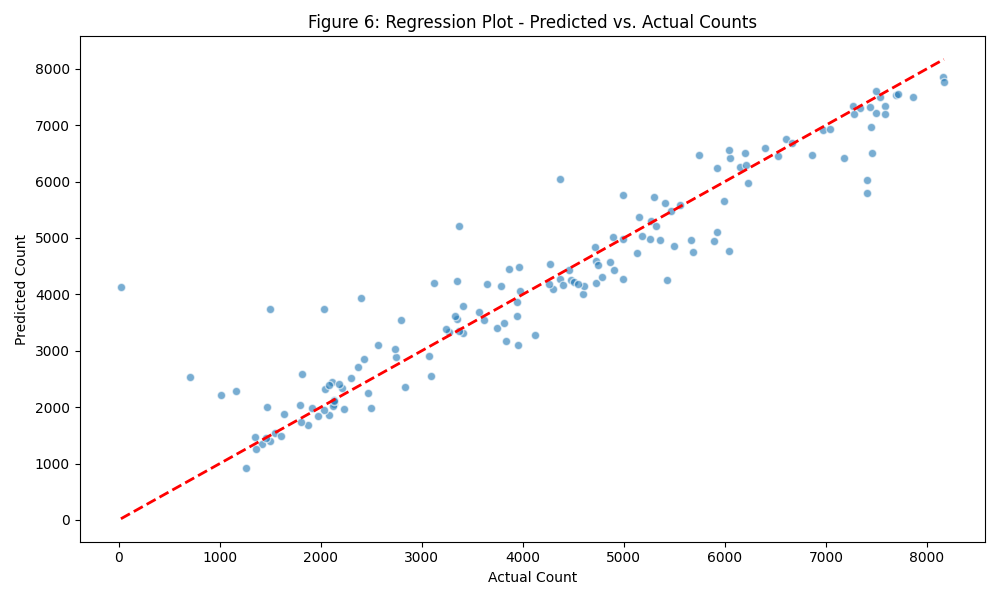
\includegraphics[width=0.7\textwidth]{11.png}
    \caption{Regression plot: Predicted vs. Actual counts.}
\end{figure}

\section{Conclusion}
Temperature (\texttt{temp}) shows the strongest positive correlation with bike usage. The Random Forest model proved highly effective, explaining approximately 88.6\% of the variance in the daily rental counts.

\end{document}